\chapter{Research Protocol} \label{ch:research-protocol}

We ultimately perform a multiscale Frangi prefilter on a subset of 201 color images of placental samples. We describe here the sample set and the preprocessing steps we take prior to performing the multiscale filter.

\section{Samples / Image Domain}\label{sec:NCS-data-set}

The 201 samples are from a larger private database provided by the National Children's Study, which had been prepared for a different study \autocite{chang2017}. These 201 samples are those that have a ground truth provided, although the actual database is much larger with many untraced samples. The placental samples were cleaned and formalin-fixed prior to their being photographed \autocite{almoussa-ucla-reu}, and their placental chorionic surface vascular networks (PCSVN) manifest as primarily dark curvilinear structures. The samples are provided as XCF files (the native project file for the image processing software GIMP) and contain four major layers.

\subsection{A Representative Sample}
The layers together give a hand tracing of the vascular network and perimeter. A sample of overlaid layers in a representative sample (with ID number ``BN0164923'') is given in \cref{fig:NCSlayers}.

\begin{figure}[p] \centering
    \subfloat[Fixed Placental Sample]{        \label{fig:NCSlayers-raw}\includegraphics[width=80mm]{{{T-BN0164923.raw}}}
        }
    \subfloat[Perimeter tracing and UCIP]{
        \label{fig:NCSlayers-P}\includegraphics[width=80mm]{{{T-BN0164923_perimeter_overlay}}}
    }\
    \subfloat[Arterial tracing]{
        \label{fig:NCSlayers-A}\includegraphics[width=80mm]{{{T-BN0164923_arteries_overlay}}}
        }
    \subfloat[Venous tracing]{
        \label{fig:NCSlayers-V}\includegraphics[width=80mm]{{{T-BN0164923_veins_overlay}}}
        }\
    \subfloat[Total Vascular Network]{
        \label{fig:NCSlayers-T}\includegraphics[width=80mm]{{{T-BN0164923_all_layers_overlay}}}
        }
    % should i use the real sample names? or obfuscate?
\caption{A representative placental sample and tracing}
\label{fig:NCSlayers}
\end{figure}

Each sample is roughly 1954x1200 pixels with some occasional variation.
In \cref{fig:NCSlayers}, we see these four layers of a characteristic sample.
\cref{fig:NCSlayers-raw} is the base image.
A cleaned, formalin-fixed placenta is placed on a table with a camera a fixed distance away,
and a ruler and penny (presumably for redundancy) are placed nearby to aid registration and
calibration of the resolution.
The resolution of each sample is roughly 46 pixels per centimeter, with some variation.
\cref{fig:NCSlayers-P} is a tracing (in green) of the perimeter of the placenta.
The umbilical cord insertion point (UCIP) is notated in yellow.
Two cyan marks are placed on consecutive centimeter markings on the ruler.
The dots are enlarged and shown as a darker blue in the figure for clarity.
\cref{fig:NCSlayers-A} and \cref{fig:NCSlayers-V} are each hand traces of the PCSVN,
  with a layer for each the arteries and veins.
These layers are simultaneously overlain on the base image in \cref{fig:NCSlayers-T},
with the arterial trace on top,
just as the arteries generally lay on top of the veins in the samples themselves.
In these traces, the coloration of each vessel corresponds its the reported diameter.
The diameters are binned into 9 discrete widths, odd integers from 3 to 19 pixels.
Vessels of smaller diameter are either binned to three or (quite frequently) left untraced.
The correspondence between pencil color and (binned) vessel width used in the tracing protocol
  is given in \cref{tab:widthcolors}.

\begin{table}
    \centering
\begin{tabular}{ccc}
    \hline
    \rule[-1ex]{0pt}{2.5ex}
    vessel width & color (hex value) & approximate color \\
    \hline 
    \rule[-1ex]{0pt}{2.5ex}
    3 pixels &  \texttt{\#ff006f} &   magenta \\                                      
    \rule[-1ex]{0pt}{2.5ex}
    5 pixels & \texttt{\#a80000}  & dark red \\                                      
    \rule[-1ex]{0pt}{2.5ex}
    7 pixels &  \texttt{\#a800ff} & purple \\                                          
    \rule[-1ex]{0pt}{2.5ex}
    9 pixel s&  \texttt{\#ff00ff}  & light pink \\
    \rule[-1ex]{0pt}{2.5ex}
    11 pixels &  \texttt{\#008aff} & blue \\                                          
    \rule[-1ex]{0pt}{2.5ex}
    13 pixels &  \texttt{\#8aff00} &   green \\                                        
    \rule[-1ex]{0pt}{2.5ex}
    15 pixels &  \texttt{\#ffc800} &  gold \\                                    
    \rule[-1ex]{0pt}{2.5ex}
    17 pixels & \texttt{\#ff8a00}  &  orange \\                                         
    \rule[-1ex]{0pt}{2.5ex}
    19 pixels & \texttt{\#ff0015}   &  bright red  \\
    \hline
\end{tabular}
\caption{Vessel Width Color Code for Manual Tracing Protocol}
\label{tab:widthcolors}
\end{table}


The task of creating these samples, in particular the tracing and estimation involved in creating \cref{fig:NCSlayers-A} and \cref{fig:NCSlayers-V} is very labor intensive--requiring between 4 and 8 hours to trace a single sample.
A closer look at many of the samples often reveals that a great deal of subjectivity in providing this ``ground truth,'' as it is not often clear what the underlying truth really is. Often it's hard to see where the vein is, vascular networks are obscured by the umbilical stem, the blood in the vessels dries unevenly or ruptures, and the vessel seems to disappear momentarily. These situations and more will be discussed in \cref{sec:NCS-dataset-issues}, where we will demonstrate how the Frangi filter reacts to these problem areas. Our efforts at the eventual task of total network completion must deal with these shortcomings and, in some circumstances, make subjective decisions like the manual tracer did.


\subsection{Knowns and Unknowns}
Since our final goal is a fully automated procedure, we wish to simply operate on the placental sample itself, without any understanding of its provided tracing (except for judging the strength of our algorithm);
our goal is to develop an algorithm that can produce a ``ground truth'' tracing similar to \cref{fig:NCSlayers-T} or \cref{fig:NCSoutput-trace} without any user intervention.

For our purposes however, we will concede and provide a limited amount of information from the tracings, namely the provided placental perimeter (shown in green in \cref{fig:NCSlayers}). In \cref{sec:perimeter-detection} we will describe a simple edge finding algorithm that allows us to estimate the perimeter in \cref{fig:NCSlayers-P}.
Unfortunately we achieve a subpar result on a small subset of images--roughly 7 of the 201 total images--using our currently implemented algorithm, and in such cases will revert to using the reported perimeter from the ground truth.

%to provide which were previously reported as being inside the plate and sometimes led to large false positives. In the case that this method 
%In developing a fully automated algorithm, it would be relatively straightforward to obtain this boundary ourselves using various techniques, such as an Active Contour Model \autocite{activecontours} or, even 
%We do use the traced placental perimeter at our own peril, however, since often there are tears in the side of the plate or large amounts of non-vascular content with large changes in height that are not adequately accounted for in the perimeter tracing.

Finally, we will consider the location of the umbilical insertion point as a ``known'', as the vessels around it are frequently impossible to see and we wish to exclude them from consideration. It is not unreasonable, however, to consider this to be a known--in future preparations of samples, we could simply require that this point be centered in image in a predictable location prior to the picture being taken.
Furthermore, we suggest that we can avoid this in the future by using an algorithm to find the umbilical cord stump and mask that region. Such an algorithm is certainly reasonable, although we were not able to implement something that worked on all images in a uniform fashion. Noise from the umbilical stump, if not addressed, will affect the fidelity of our filter. We will discuss this further in \cref{sec:NCS-dataset-issues}.

\section{Data Cleaning and Preprocessing}

Building a sample suitable for use in our algorithm from \cref{fig:NCSlayers} is relatively simple. We  zero  outside the boundary of the plate (so as to not waste computational time calculating the differential geometry of a ruler, say), and also generate a binary mask to identify the plate. Finally, our vessel layers are combined and given as a binary trace, which we will use later for scoring. An example of the preprocessed samples used by the algorithm are given in \cref{fig:exampleNCSoutput}.

These procedures are performed automatically on the 201 images in our data set using a custom GIMP plug-in, which performs various ``bucket fill'' operations, layer mergings, and thresholdings.
%For completeness sake, this plug-in (and an associated Scheme script which turns it into a batch operation) can be found in the Appendix.

\begin{figure}\label{fig:exampleNCSoutput}     \centering
    \subfloat[Background mask (in white)]{
        \label{fig:NCSoutput-mask}\includegraphics[width=80mm]{{{T-BN0164923.mask}}}
    }
    \subfloat[Sample with background removed]{
        \label{fig:NCSoutput-base}\includegraphics[width=80mm]{{{T-BN0164923}}}
    } \\
    \subfloat[Grayscale]{
        \label{fig:NCSoutput-gray}\includegraphics[width=80mm]{{{T-BN0164923.L}}}
    }
    \subfloat[Trace / ``Ground Truth'']{
        \label{fig:NCSoutput-trace}\includegraphics[width=80mm]{{{T-BN0164923.trace}}}
    }
    \caption{Preprocessed files from an NCS sample}
\end{figure}

    As a point of technicality, the grayscale image in \cref{fig:NCSoutput-gray} is not actually produced directly by the extractor plug-in, but created when the 3 channel RGB image \cref{fig:NCSoutput-base} is imported at the start of the algorithm. This grayscale conversion is simply done for ease of analysis on the sample: although the Frangi filter is designed for arbitrary $N$-dimensional input \autocite{frangi-paper}, an image with three color channels does not have 3 spatial dimensions. We therefore simply combine the information in three channels using the well-known and oft-implemented ITU-R 601-2 luma , or ``luminance'' transform \autocite{scipy}:
    
    \begin{equation} \label{eq:luma_transform}
    L =  \frac{299}{1000}\ R + \frac{587}{1000}\ G + \frac{114}{1000}\ B
    \end{equation}
    It should be noted that this choice is not requisite--several other attempts have opted to use the image's green channel instead \autocite{almoussa-ucla-reu} and \autocite{huynh2013filter}. Preliminary and periodical rechecking has not indicated that such a conversion has any benefit over the luminance transformation for our image domain, although other placental samples with a different preparation method or color profile might benefit from it.

\subsection{Placental Perimeter Detection and Background Masking} \label{sec:perimeter-detection}
\begin{figure}     \centering
  \subfloat[Raw (traced mask)]{
    \includegraphics[width=0.24\textwidth]{{{cut_demo_new_cimg_gt}}}
  }
  \subfloat[Raw (watershed mask)]{
    \includegraphics[width=0.24\textwidth]{{{cut_demo_new_cimg_ws}}}
  } %\\
  \subfloat[$\Vmax$ (traced mask)]{
    \includegraphics[width=0.24\textwidth]{{{cut_demo_new_f_gt}}}
  }
  \subfloat[$\Vmax$ (watershed mask)]{
    \includegraphics[width=0.24\textwidth]{{{cut_demo_new_f_ws}}}
  }\\[12pt]
  \caption{Automated placental perimeter detection}
  \label{fig:cut-demo}
\end{figure}

As mentioned above, expect for a few small images, we estimate the perimeter of the placental plate from the raw image, rather than using the ground truth's traced perimeter. Most notably, the placental plate often includes includes a small V-shaped cuts in the placental plate.
The traced placental perimeter often overlooks these regions and opt for a more convex shape.
In \cref{fig:cut-demo}, we showcase the effect of using our automated approach versus using the ground truth mask. The first two images demonstrate the Notably, this prevents the white background leading to false positives at the edge of the cut.
To find the placental plate,we take the gradient of the raw sample's green channel with a very small scale $\sigma=.01$ to identify very small and sharp edges. We then mark the top right pixel, which is certainly outside the placental plate, with a background marker, and we label any points where the gradient is above its mean value as foreground. We then perform a watershed of the gradient given these markers and then perform a binary erosion of the result with radius 15 to regularize the result \autocite{skimage} \autocite{DIPGW}. From this, we grab the largest foreground object, which will inevitably be the placental plate. Unfortunately, there are 7 of the 201 samples for which this procedure fails, typically due to poor contrast at the edge of the placental plate. In the case of these samples, we revert to simply using the traced outline of the placenta as given by the tracing protocol.

    \subsection{Boundary Dilation} \label{sec:boundary-dilation}
    
    All images are grayscale, $M,N$ pixels as a masked array, where pixels outside of the placental region are masked so they will not be considered by the algorithm. However, some standard
    implementations of algorithms, namely \textrm{numpy.gradient and scipy.signal.convolve2d} are not designed to handle masked regions. Although it would be potentially useful to adapt such methods in a way to, say, calculate a gradient or perform a convolution by a ``reflection'' across an arbitrary closed boundary (as opposed to the edge of the image matrix), we opted instead to ``zero out'' unwanted background pixels and simply exclude affected areas from consideration. This exclusion could be achieved by
    simply dilating the mask, but we opt to achieve it in a much more resource efficient manner: we iterate through an array of indices for the image where the boundary occurs and simply extend the mask $R$ pixels in each direction (like a giant plus sign). Since the boundary of the placental plate forms a closed loop, the effect is very similar to convolving with a disk of radius $R$, but is much faster.
    
    \begin{figure} 
        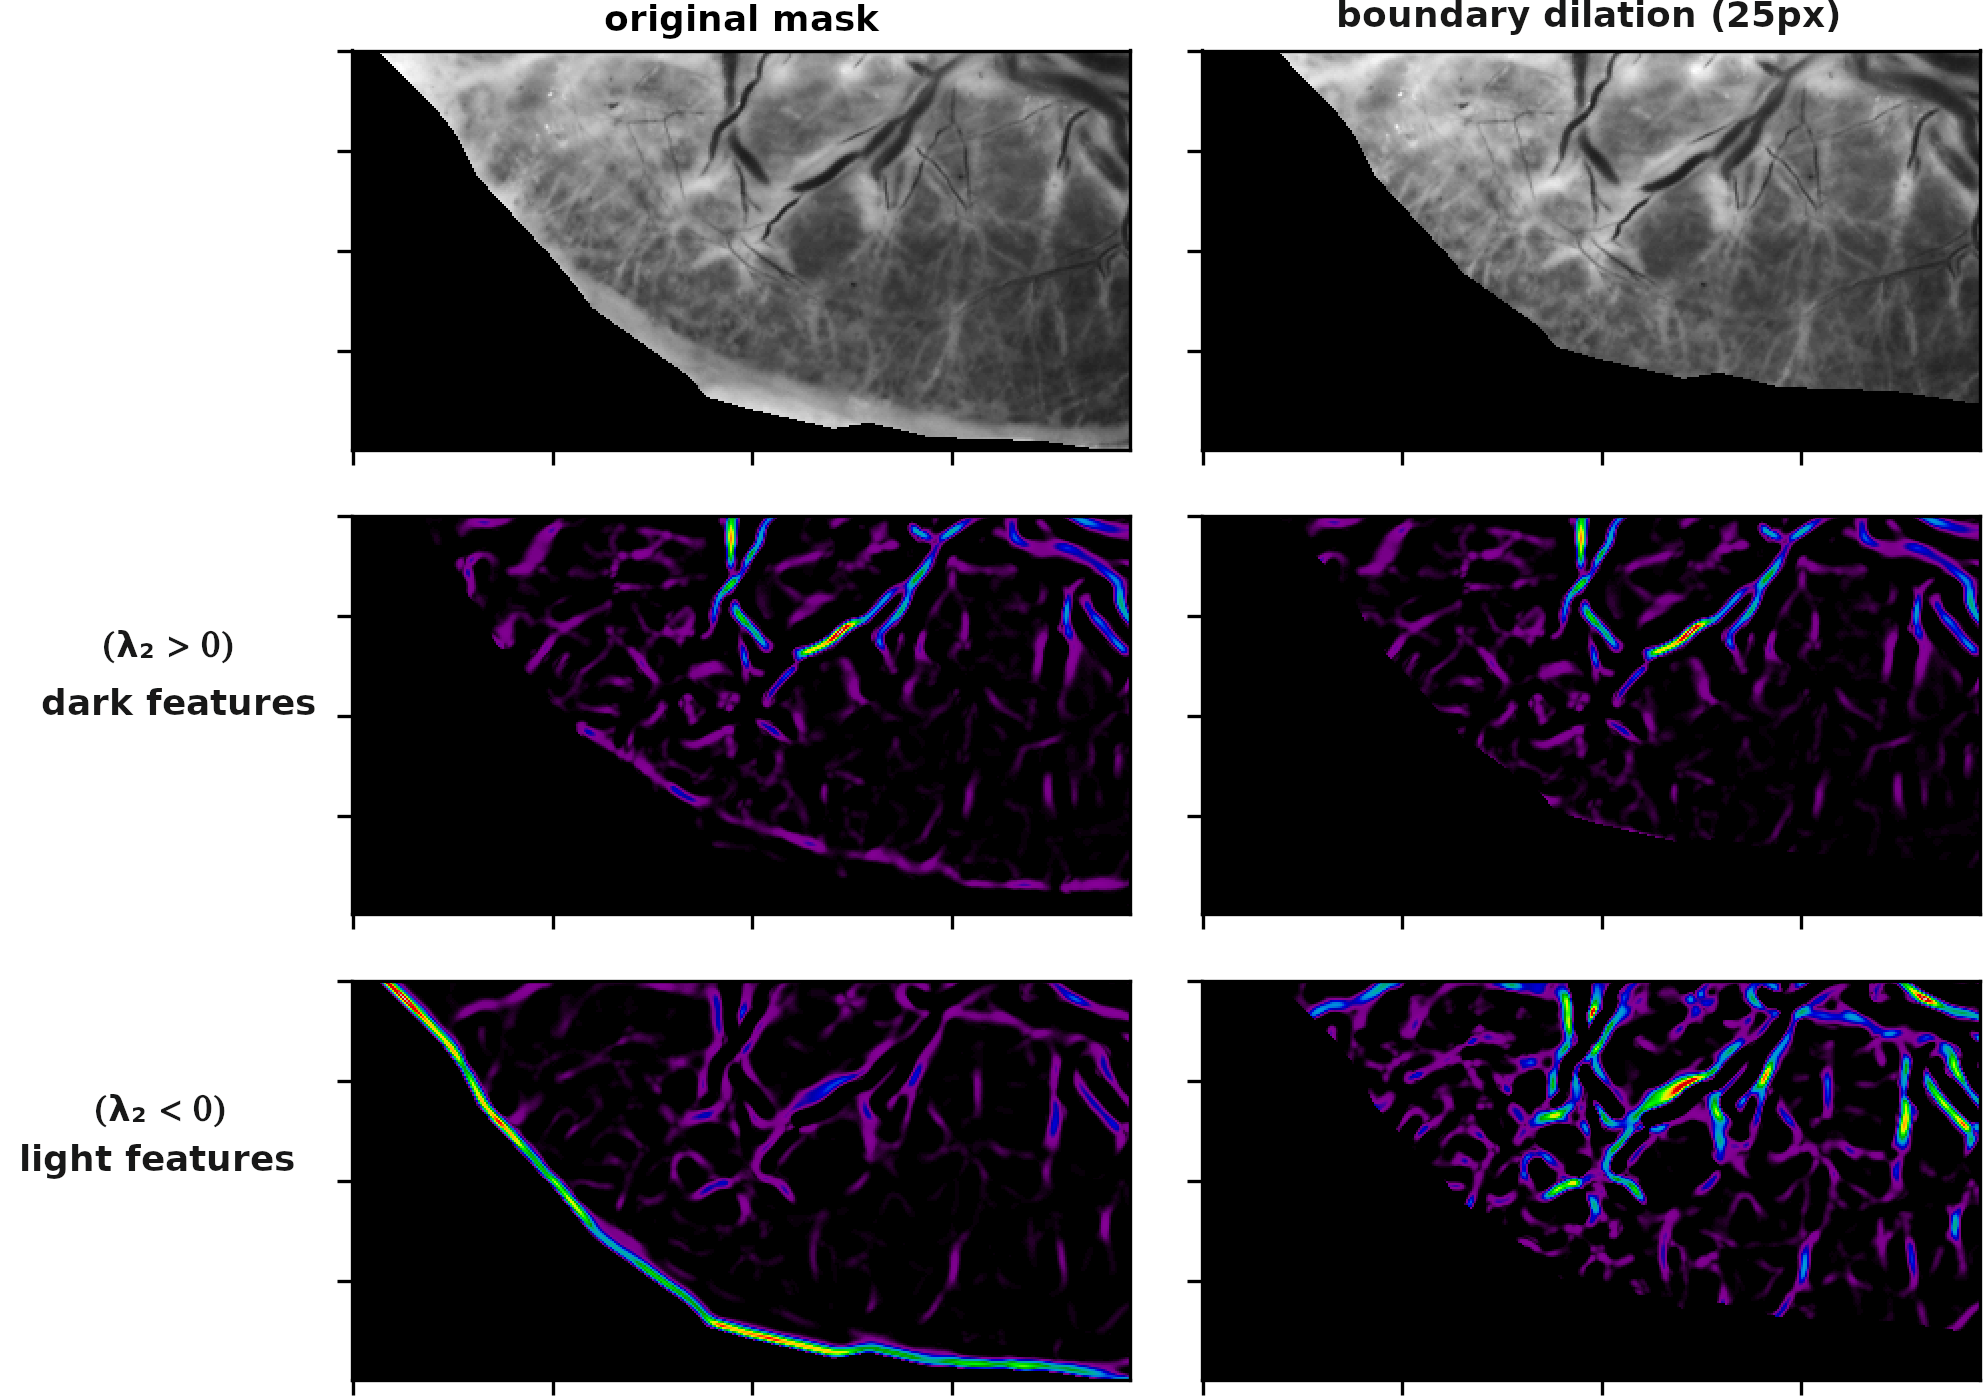
\includegraphics[width=\textwidth]{boundary_dilation_demo_labels}
        \caption{Effect of boundary dilation on Frangi responses}
        \label{fig:boundary-demo}
    \end{figure}
    
    \cref{fig:boundary-demo} shows the effect of this so-called ``boundary dilation.'' 
    We show the output of the Frangi filter with $\sigma=3$. A border radius of $25$ is chosen to exaggerate the effect.
    The first row shows the unaltered boundary of the sample (left) and
        the sample after boundary dilation (with radius dilation of 25 pixels).
    The second row shows the Frangi vesselness measure at single scale ($\sigma=3$) where \textrm{DARK\_BG=False} to target dark curvilinear structures performed on the altered sample (left) and the boundary dilated sample (right). Removing an unnecessary part of
    the placental plate prevents a small response to a non-vascular yet mildly curvilinear
    background feature from appearing.
    The third row of \cref{fig:boundary-demo} shows the Frangi vesselness measure at the same scale ($\sigma=3$) when we are probing for bright curvilinear structures (i.e.
    \textrm{DARK\_BG=True}). Here, wherever the very edge of the placental plate is *any* brighter than adjacent interior, a very large Frangi response will occur, as seen on the left. Dilating the boundary completely avoids this issue, as seen by the figure on the right. Thus we prevent a visual artifact that is present in much prior work on this problem \autocite{huynh2013filter,almoussa-ucla-reu}.

    It should be noted that, while the figure on the right shows a much larger interior response, this is simply because the intensity of the output in each of these
    images is being independently scaled between the minimum and maximum intensity in the image. However, we argue that this is an appropriate and desired depiction of the situation, as we will frequently consider only the relative maxima of Frangi response per scale in our analysis.
    
    We end our discussion by noting that we perform this boundary dilation within the
    Frangi algorithm itself when we set the structureness parameter $\gamma$ as half of the maximum Hessian norm found at that scale--this ensures that the maximum occurs sufficiently away from the boundary of the plate, and does not occur from a noise phenomenon.

    
    
    Sometimes there are small cuts that appear on the side of the placental plate, which can lead to large filter responses. We would like to filter these out to eliminate false positives in any way we can. These places are identified somewhat reliably by the tracing protocol with a blue dot. We perform a morphological watershedding in this area in an attempt to add this area to the mask.
    The threshold for the watershed is ultimately based on the background value of the blue dot; if this is incorrectly placed (or anything else weird happens), we can manually opt to simply remove a large area from consideration from the plate, as we do the umbilicial cord insertion point. This is demonstrated in \cref{fig:cut-demo}. From left to right, we have the original masked placental sample, the cut mark notated on the perimeter layer, the improved mask after watershedding, and finally, the ``scorched earth'' approach in case the previous attempt failed. In few additional cases, neither approach is adequate. We again will stress that a fully automated algorithm would have no knowledge of our traced perimeter (as in \cref{fig:NCSlayers-P} or the second from left image in \cref{fig:cut-demo}), so we anticipate a fully automated method of handling that problem should also be able to correct for these ``cuts'' as well.

		
		    \subsection{Deglaring}
    
    Despite best efforts when harvesting samples, a select number of the placental samples exhibit substantial glare, which leads to inaccuracies in identifying curvilinear content. Our protocol for deglaring is analogous to that performed in \autocite{almoussa-ucla-reu} and \autocite{huynh2013filter}. Unfortunately, the method relied upon by those previous papers (\textrm{MATLAB}'s \textrm{imfill}, which relies on inpainting by solving the Dirichlet problem for masked regions) was not immediately available in a Python environment. Instead, we used an already implemented inpainting algorithm, \textrm{scikit-image}'s \textrm{inpaint\_biharmonic()}, which should be expected to achieve similar results, albeit at the expense of processing time.
    
    The function \textrm{inpaint\_biharmonic} is based on \autocite{damelin2018surface}, and relies on solving the biharmonic equation i.e. $\nabla \nabla f = 0$
    for the surface $f$ subject to boundary conditions (as
    compared to \textrm{imfill}'s solving the Laplace equation $\nabla f = 0$ in regions marked as glare.
    
    The method for deciding what is considered glare is similar to \autocite{almoussa-ucla-reu}, in which we
    consider any intensities close the maximum intensity in the image (Almoussa et al. used $80\%$ of max intensity, and we use $175/255 \approx 68\%$). This threshold is unfortunately dependent on the image domain.
` filter according to \cref{ch:unifrangi} and \cref{ch:multifrangi}. We use these to provide a couple examples of estimating the PCSVN network. The entire decision tree can be shown in the outline below. We follow the procedure for \cref{ch:segmentation}. For our analysis of the Frangi filter apart from segmentation we shall stop before step (C). For the decision tree, please refer to \cref{app:decisiontree}.
%    
%    \begin{spacing}{1}
%    \begin{small}
%    \begin{verbatim}
%For each sample:
%
%A) Preprocessing
%  1) Find placental border
%  	a) Gradient of green channel for small sigma=.01
%  	b) Watershed outside against above gradient mean
%  	c) erode these points, radius=15
%  	d) Identify largest object in watershed threshold
%  2) RGB to single channel via Luminance Transform
%  3) Glare removal
%    a) Mask glare (threshold at *175/255*)
%    b) Dilate glare mask with radius=2
%    c) Inpaint glare
%      + Hybrid inpainting, with size threshold *32*
%      . Biharmonic inpainting
%      . Median value of boundary
%  4) Dilate around UCIP, add to mask (radius=50)
%B) Multiscale Frangi filter
%  1) Set parameters
%    a) Scales
%      = n_scales (default: *20*)
%      = log_range (default *[-1.5, 3.2]*), log base 2
%      -> scales
%    b) Beta = 0.1, Gamma = 1.0 (or alternate parametrization)
%    d) Dilate mask per scale (20 pixels)
%  2) For each sigma: compute Uniscale Frangi Filter
%    a) gauss blur image with discrete Gaussian kernel FFT
%    b) take gradient across each axis of blurred image;
%       take gradient across each axis of gradient
%       -> (Hxx, Hxy, Hyy)
%    c) Find eigenvalues of hessian at each point (using np.eig)
%       and sort by absolute magnitude 
%    d) Calculate Frangi Vesselness Measure
%  3) Split positive and negative strain.
%  3) Merge each result, reserve positive and negative stacks
%C) Estimate PCSVN
%  1) Approximate using strategy
%    a) Calculate Vmax above high fixed threshold alpha=0.3
%    b) Calculate Vmax above lower fixed threshold alpha=0.2
%    b) Threshold scalewise at 95th nonzero-percentile
%    c) Threshold scalewise at 98th nonzero-percentile
%    d) Margin adding algorithm with high fixed threshold
%  2) Compare to ground truth trace to obtain confusion matrix
%  3) Calculate MCC score and precision
%\end{verbatim}
%    \end{small}
%\end{spacing}
